%%%%%%%%%%%%%%%%%%%%%%%%%%%%% Define Article %%%%%%%%%%%%%%%%%%%%%%%%%%%%%%%%%%
\documentclass{article}
%%%%%%%%%%%%%%%%%%%%%%%%%%%%%%%%%%%%%%%%%%%%%%%%%%%%%%%%%%%%%%%%%%%%%%%%%%%%%%%

%%%%%%%%%%%%%%%%%%%%%%%%%%%%% Using Packages %%%%%%%%%%%%%%%%%%%%%%%%%%%%%%%%%%
\usepackage{geometry}
\usepackage{graphicx}
\usepackage{amssymb}
\usepackage{amsmath}
\usepackage{amsthm}
\usepackage{empheq}
\usepackage{mdframed}
\usepackage{booktabs}
\usepackage{lipsum}
\usepackage{graphicx}
\usepackage{color}
\usepackage{psfrag}
\usepackage{pgfplots}
\usepackage{bm}
%%%%%%%%%%%%%%%%%%%%%%%%%%%%%%%%%%%%%%%%%%%%%%%%%%%%%%%%%%%%%%%%%%%%%%%%%%%%%%%

% Other Settings
% LTeX: language=es
\graphicspath{ {./resources/} }

%%%%%%%%%%%%%%%%%%%%%%%%%% Page Setting %%%%%%%%%%%%%%%%%%%%%%%%%%%%%%%%%%%%%%%
\geometry{a4paper}

%%%%%%%%%%%%%%%%%%%%%%%%%% Define some useful colors %%%%%%%%%%%%%%%%%%%%%%%%%%
\definecolor{ocre}{RGB}{243,102,25}
\definecolor{mygray}{RGB}{243,243,244}
\definecolor{deepGreen}{RGB}{26,111,0}
\definecolor{shallowGreen}{RGB}{235,255,255}
\definecolor{deepBlue}{RGB}{61,124,222}
\definecolor{shallowBlue}{RGB}{235,249,255}
%%%%%%%%%%%%%%%%%%%%%%%%%%%%%%%%%%%%%%%%%%%%%%%%%%%%%%%%%%%%%%%%%%%%%%%%%%%%%%%

%%%%%%%%%%%%%%%%%%%%%%%%%% Define an orangebox command %%%%%%%%%%%%%%%%%%%%%%%%
\newcommand\orangebox[1]{\fcolorbox{ocre}{mygray}{\hspace{1em}#1\hspace{1em}}}
%%%%%%%%%%%%%%%%%%%%%%%%%%%%%%%%%%%%%%%%%%%%%%%%%%%%%%%%%%%%%%%%%%%%%%%%%%%%%%%

%%%%%%%%%%%%%%%%%%%%%%%%%%%%%%% Plotting Settings %%%%%%%%%%%%%%%%%%%%%%%%%%%%%
\usepgfplotslibrary{colorbrewer}
\pgfplotsset{width=8cm,compat=1.9}
%%%%%%%%%%%%%%%%%%%%%%%%%%%%%%%%%%%%%%%%%%%%%%%%%%%%%%%%%%%%%%%%%%%%%%%%%%%%%%%

%%%%%%%%%%%%%%%%%%%%%%%%%%%%%%% Title & Author %%%%%%%%%%%%%%%%%%%%%%%%%%%%%%%%
\title{Proyecto Final de Informática}
\author{Integrantes}
%%%%%%%%%%%%%%%%%%%%%%%%%%%%%%%%%%%%%%%%%%%%%%%%%%%%%%%%%%%%%%%%%%%%%%%%%%%%%%%

\begin{document}
    \maketitle
    
\section{Programa de Inicio}

El programa de inicio utiliza un ciclo \emph{do} junto a una variable booleana \emph{run}, de esta manera se obtiene a un programa que continuara ejecutando a no ser que el valor de \emph{run} sea falso. 

\begin{figure}[h]
    \centering
        \centering
    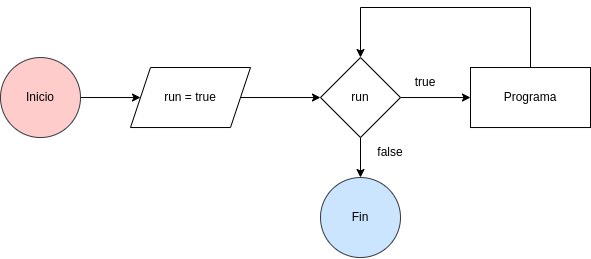
\includegraphics[width=8cm]{loop_inicio}
    \centering
        \centering
        \caption{Loop Principal del Programa}
\end{figure}

Acá se le presenta al usuario una lista de programas disponibles y se captura la opción ingresada, este valor se evalúa con una estructura de control \emph{switch} para ejecutar cada ejercicio.

\begin{figure}[h]
    \centering
    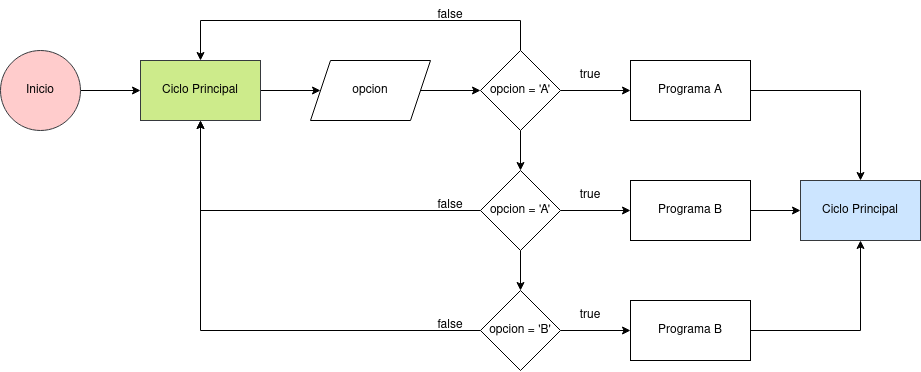
\includegraphics[width=8cm]{switch_programa}
    \caption{Switch Selecionador de Programas}
\end{figure}

\section{Primer Programa}

El primer programa empieza capturando las 3 variables: \emph{a}, \emph{b} y \emph{c}, de tipo \emph{double} para no perder precisión al momento de calcular el área del triángulo. Estas variables son entonces evaluadas en un condicional para verificar si una de ellas es negativa o igual a 0, de ser verdad entonces se muestra el error ``¡Solo se aceptan valores positivos!'', de ser falso se continúa con otro condicional para evaluar si los valores ingresados crean un triángulo: \emph{(a + b) > c}, de ser falso se muestra el error: ``¡Los valores ingresados no crean un triángulo!''. Con estos valores ya evaluados se utiliza la \emph{fórmula de Herrón} para obtener el área del triángulo.

\begin{figure}[h]
    \centering
    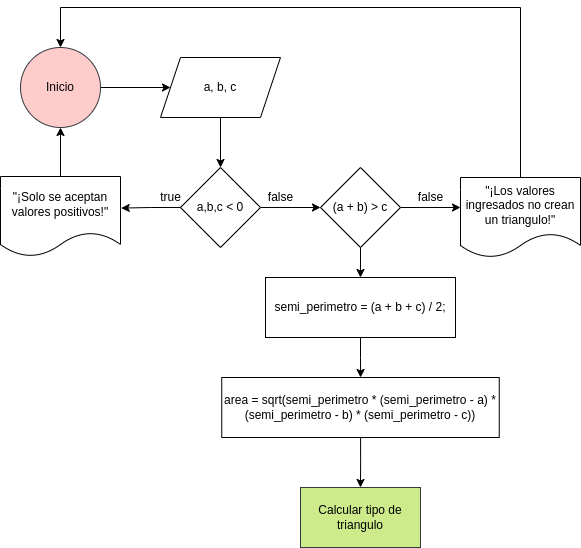
\includegraphics[width=8cm]{triangulo_area}
    \caption{Programa Calculador de Área de un Triángulo}
\end{figure}

Con el cálculo del área completo, se evalúa el tipo de triángulo con las medidas ingresadas.

\begin{figure}[h]
    \centering
    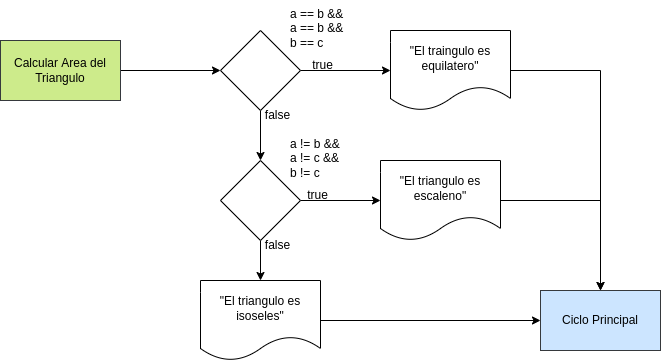
\includegraphics[width=8cm]{triangulo_tipo}
    \caption{Programa Calculador del Tipo de Triangulo}
\end{figure}

\end{document}
